\documentclass[../main.tex]{subfile}

\begin{document}

\tikzset{/tkzmkangle/mark=none}

\topictitle{Basics}

\sectitle{Definitions}

\begin{figure}[H]
	\begin{minipage}{0.45\linewidth}
	\begin{center}
	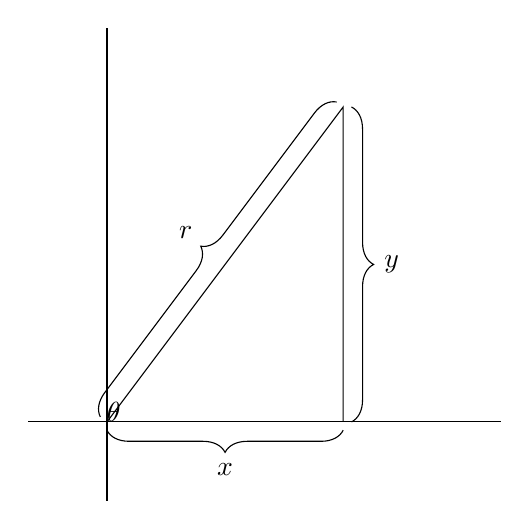
\begin{tikzpicture}
		\coordinate (O) at (0,0);
		\coordinate (A) at (3,4);
		\coordinate (xDrop) at (3,0);

		\draw (-1,0) -- (5,0);
		\draw (0,-1) -- (0,5);

		\draw (O) -- (A) -- (xDrop);

		\draw[decorate, decoration={brace, amplitude=8pt, raise=3pt}]
			(O) -- node[above, yshift=2mm, xshift=-5mm] {$r$} (A);
		\draw[decorate, decoration={brace, amplitude=8pt, raise=3pt, mirror}]
			(O) -- node[below, yshift=-4mm] {$x$} (xDrop);
		\draw[decorate, decoration={brace, amplitude=8pt, raise=3pt, mirror}]
			(xDrop) -- node[right, xshift=4mm] {$y$} (A);

		\tkzMarkAngle(xDrop,O,A);
		\tkzLabelAngle[pos=0.7](xDrop,O,A){$\theta$};
	\end{tikzpicture}
	\end{center}
	\end{minipage}\hfill
	\begin{minipage}{0.5\linewidth}
		\setlength{\parskip}{1em}
		Cartesian coordinates are specified as $(x, y)$. Polar coordinates are specified as $(r; \theta)$. They are related like so:
		\begin{empheq}[box=\rememberBox]{align*}
			\displaystyle
			r^2 &= x^2 + y^2\\
			\tan\theta &= \frac{y}{x}\\
			r\cos\theta &= x\\
			r\sin\theta &= y
		\end{empheq}

		These equations can be used to convert between polar and Cartesian coordinates.
	\end{minipage}
\end{figure}

\sectitle{Conventions}

Desmos and GeoGebra both draw polar coordinates with negative $r$ values in the opposite direction, with the same absolute distance from the origin.

The book and the A Level exams use a different convention where negative $r$ values are discarded and counted as 0.

\end{document}
